%Her beskrives den arbejdsmetode, der har været anvendt i projektet, f.eks. Scrum.
\chapter{Development process}

\section{ASE model}
This project was developed using the ASE model, like all our previous projects at the university. Figure~\ref{fig:asemodel} shows the structure of the model.

\begin{figure}[H]
\centering
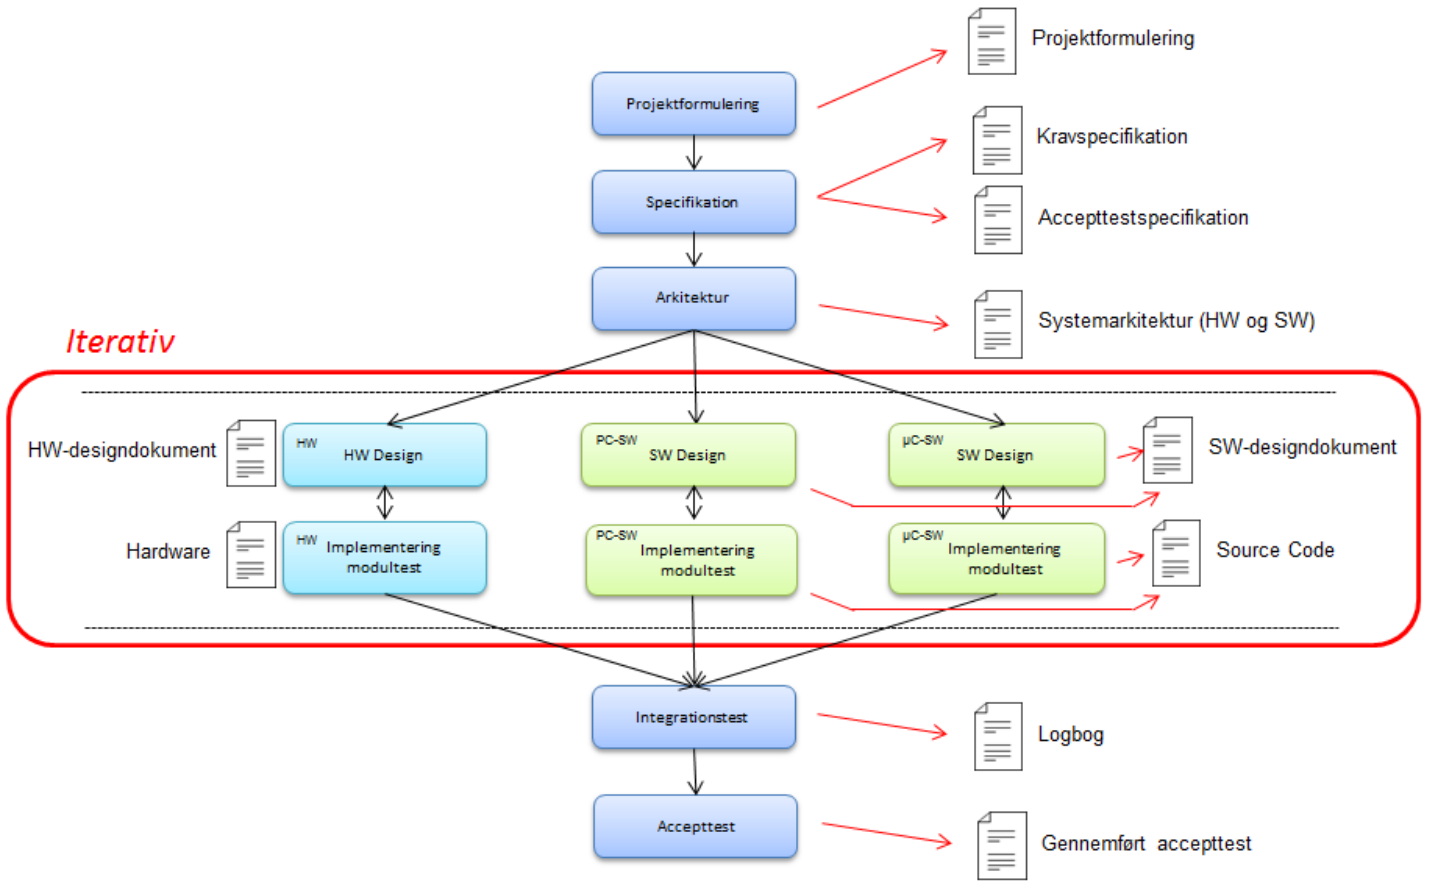
\includegraphics[width=1\linewidth]{ASE_model}
\caption{The ASE development model}
\label{fig:asemodel}
\end{figure}

 As seen, the project development proceeds linearly from problem definition to requirements specification, and then architecture. 
 
 After this, development begins, and the system is designed and tested iteratively. When all components have been developed and verified, integration tests are run to verify that the components work together.
 
  Finally, the acceptance test (written after the architecture has been completed) is run, and it is verified that the system behaves as expected from the requirements specification.
  
  Using this model is very intuitive after having used it in several projects, and it ensures that due diligence is exercised instead of jumping into development prematurely.
  
  \section{SCRUM}
  SCRUM is an agile development process that has seen successful use in a wide variety of organizations for the past twenty years or so.
  
  A modified version of SCRUM was used during development. Since the team consisted of only two members, a full SCRUM approach seemed unnecessarily time-consuming, so only the elements of SCRUM that were deemed relevant were incorporated into the development process, such as artefacts, and Time boxes. 
  
  During certain parts of development it was essential that certain modules were finished before others could be started, which naturally led to several "mini-sprints". A batch of tasks would complete, be reviewed, then be finished, and new tasks were possible to begin, building on top of the finished ones.
  
  In this project, both members of the team were Development Team and Product Owner, as well as SCRUM Master, and meetings were held rather informally, usually after modules finished, and there were problems to discuss and solve. 